% Author: CSC Officers
\documentclass[11pt]{article}
\usepackage[margin=0.7in]{geometry}
\usepackage{listings}   %
\usepackage{needspace}  %
\usepackage{color}      %
\usepackage{ifthen}     % 
\usepackage{graphicx}   %
\usepackage{../includes/csc}        %
\usepackage{tikz}       %
\usetikzlibrary{shapes} %
\usepackage{tabularx}   % for helping matchtabular (matching questions)
\usepackage{textcomp}	% So our quotes in code don't look like shit
\usepackage{longtable}
\usepackage{multicol}
\usepackage[usenames,dvipsnames]{pstricks}
\usepackage{epsfig}
\setlength{\columnsep}{12em}

\lstset{ %
basicstyle=\footnotesize\ttfamily,       % the size of the fonts that are used for the code
numbers=left,                   % where to put the line-numbers
stepnumber=1,                   % the step between two line-numbers. If it's 1 each line will be numbered
numbersep=5pt,                  % how far the line-numbers are from the code
showspaces=false,               % show spaces adding particular underscores
showstringspaces=false,         % underline spaces within strings
tabsize=4,		                % sets default tabsize to 4 spaces
language=C,
upquote=true,
columns=fixed
}

\ifthenelse{\isundefined{\isAnswerKey}}
{
    \newenvironment{answer}{\large\lstset{basicstyle=\tiny\ttfamily}\color{white}}{}
}
{
    \newenvironment{answer}{\large\lstset{basicstyle=\large\ttfamily}\color{red}}{}
}

% ----- Start matchtabular definition -----
\newcounter{matchleft}
\newcounter{matchright}
\newenvironment{matchtabular}{%
  \setcounter{matchleft}{0}%
  \setcounter{matchright}{0}%
  \tabularx{\textwidth}{%
    >{\leavevmode\hbox to 1.5em{\stepcounter{matchleft}\arabic{matchleft}.}}X%
    >{\leavevmode\hbox to 1.5em{\stepcounter{matchright}\alph{matchright})}}X% 
    }%
}{\endtabularx}
% ----- End matchtabular definition -----

\title{CSCI-243 Final Exam Review}
\author{Computer Science Community}
\date{\today}

\makeatletter
\let\thetitle\@title
\let\theauthor\@author
\let\thedate\@date
\makeatother

\begin{document}
	\header 

	\begin{enumerate}
		\section*{History \& Language Paradigms}
		\item Explain the relationship between machine language, assembly language, and high level languages.\\
\begin{answer}
\small{\textbf{Machine language} is a set of instructions that is executed directly as-is by the computer's CPU itself. This is considered the lowest level representation of a computer program, and, while it is possible to program directly in machine code, it is highly tedious and error prone, making higher level languages favorable. Writing machine code is typically only done when troubleshooting a system or when implementing extreme optimization.\\
\textbf{Assembly language} is also considered a low-level programming language, and, in particular, assembly usually has a near 1:1 relationship between the assembly code and the architechure's machine code instructions. Assembly languages are specific to a computer's architechture - for example, assembly code you write for your phone (almost certainly) wouldn't work on your laptop. An example of an assembly language is MIPS. Programming in assembly language (and lower) is commonplace in embedded systems work.
\\
Finally, \textbf{high level languages} are, in general, designed to be portable across many different architechtures. What separates the high level languages from their lower level counterparts is that, due to this fact, they require compiling, which translates your high-level code into a form which the machine can understand (which varies by architechture.) When people talk about programming languages, they are most often referencing one of the high level languages, unless otherwise specified. High level languages include C and C++, Python, and Java.}
\end{answer}

		
		\item \begin{enumerate}

\item List a difference between imperative/procedural programming and object-oriented programming.

\begin{answer}
In procedural programming, the program is a flat collection of global functions and variables. In object-oriented programming, functions and variables are grouped into classes, where they can be encapsulated from other classes.
\end{answer}


\item List a difference that functional programming has from procedural or object-oriented programming.

\begin{answer}
In functional programming, functions return values based solely on their input, and do not affect the state of any other data. Rather than programs being composed of statements executed in sequence, programs are composed of function applications which produce the desired output.
\end{answer}

\end{enumerate}


		\section*{Basic C}
		\item Examine the following program:

\begin{verbatim}
#include <stdio.h>

int main(int argc, char* argv[]) {
    int number = atoi(argv[1]);      // atoi parses int from str
    int found;
    do {
        int i;
        found = 1;
        --number;
        for (i = 2; i < number; ++i) {
            if (!(number % i)) {
                found = 0;
                break;
            }
        }
    } while (!found);
    printf("%d", number);
    return 0;
}
\end{verbatim}

\begin{enumerate}

\item What does this program do? What is the output of \texttt{./a.out 10}? Step through the program execution if it helps.

\begin{answer}
This program finds the largest prime number less than the first command line argument. \texttt{./a.out 10} sets \texttt{number} to 10. The first iteration of the do-while loop decrements \texttt{number} to 9, then the for loop tests all integers between 2 and 8 inclusive for one that divides into 9 evenly. It finds that \texttt{9 \% 3} equals 0, so \texttt{!(9 \% 3)} equals 1. Since 1 is not equal to 0, it enters the if statement and breaks out of the for loop. It continues the do-while loop, decrements \texttt{number} to 8, and finds 2 divides into 8 evenly. \texttt{number} is then decremented to 7, and all integers from 2 to 6 inclusive are tested to check if they divide into 7 evenly. None of them do (because 7 is prime), so the if statement isn't executed. \texttt{found} is now 1 at this point, making \texttt{!found} equal 0, which stops the loop, and 7 is then printed.
\end{answer}



\item Why can we write \texttt{if (!(number \% i))} instead of \texttt{if (number \% i == 0)}? (These statements are equivalent.)

\begin{answer}
If statements in C check whether their condition is not equal to 0, rather than if they are equal to a dedicated "true" value. If \texttt{number \% i} is 0 (that is, \texttt{number} is a multiple of \texttt{i}), then \texttt{!(number \% i)} will equal 1, which is not equal to 0, so the if condition will be satisfied. Comparison operators all produce 0 or 1, so here, \texttt{number \% i == 0} would evaluate to \texttt{0 == 0}, which evaluates to 1.
\end{answer}


\newpage
\item Rewrite the code using while loops in place of the do-while loop and the for loop.

\begin{answer}
\begin{verbatim}
#include <stdio.h>

int main(int argc, char* argv[]) {
    int number = atoi(argv[1]);      // atoi parses int from str
    int found = 0;
    while (!found) {
        int i; 
        found = 1;
        --number;
        i = 1; // Start one below the desired initial value, as i will be immediately incremented.
        while (i < number) {
            ++i;
            if (!(number % i)) {
                found = 0;
                break;
            }
        }
    }
    printf("%d", number);
    return 0;
}
\end{verbatim}

Note that we place the increment statement at the top of the loop body because if the loop body contained a \texttt{continue} statement, the increment statement will always be executed, unlike if the increment statement were placed at the bottom. Because this code does not include a \texttt{continue} statement, initializing \texttt{i} to 2 and placing the increment statement at the bottom of the loop body will also produce the correct behavior.
\end{answer}

\end{enumerate}


		\section*{I/O}
		\item Write a program that searches a file for a provided number on \texttt{stdin}.
Print out any errors on \texttt{stderr}.
Example:

\begin{lstlisting}
$ fileSearch file.txt
> 234
found: 234
\end{lstlisting}

\begin{answer}
\begin{lstlisting}
#include <stdio.h>
#include <stdlib.h>

int main(int argc, char* argv[]) {
	if(argc != 2) {
		fprintf(stderr, "Usage: fileSearch <filename>");
		exit(EXIT_FAILURE);
	}
	FILE* handle = fopen(argv[1], "r");
	if(!handle) {
		perror("fopen failed:");
		exit(EXIT_FAILURE);
	}
	int input = 0;
	scanf("\%d", \&input);
	int check = 0;
	while(fscanf(handle, "\%d", \&check) != EOF) {
		if(check == input) {
			printf("found: \%d", input);
			exit(EXIT_SUCCESS);
		}
	}
	fclose(handle);
	printf("\%d not found", input);
	return EXIT_SUCCESS;
}
\end{lstlisting}
\end{answer}


		\item \begin{enumerate}
\item The following program is intended to read a text file and outputs (as binary data) the number of characters (including new lines) in each line to a file. However, there is a problem with the code the way it is currently written. Find the problem and explain how to fix it. Note: The code is compiled and linked using GCC.

\lstinputlisting{code/getline_binary_io.c}

\begin{answer}
The signature of \texttt{getline} is \texttt{ssize\_t getline(char** lineptr, size\_t* n, FILE* stream)}. If \texttt{*lineptr} is \texttt{NULL} and \texttt{*n} is 0, then \texttt{getline} will dynamically allocate a C string containing the next line of \texttt{stream} (including the new line character), and set \texttt{*lineptr} to this C string, and \texttt{*n} to the size of this new stream. It returns the size of the string read. If the \texttt{*lineptr} given to the function is not \texttt{NULL}, then it expects \texttt{*n} to be the length of \texttt{*lineptr}, and it will attempt to use \texttt{*lineptr} to hold the next line if it can fit, otherwise it will use \texttt{realloc} to allocate enough space for it to fit. This program does not use \texttt{getline} correctly, and causes a type error when compiling. See the answer of the next question for how to fix this problem.
\end{answer}

\newpage
\item Rewrite the code so that it outputs the data using binary streams instead.
\end{enumerate}

\begin{answer}
\lstinputlisting[basicstyle=\small]{code/getline_binary_io_correct.c}
\end{answer}

			
		\section*{C Preprocessor}
		\item What is the value of \texttt{i}?
\begin{verbatim}
#define THING1 40
#define THING2 32

#if THING1 < THING2
#define THING3 5
#elif THING2 < THING1
#define THING3 6
#else
#define THING3 7
#endif

int i = THING3;
\end{verbatim}
\begin{answer}
6
\end{answer}

		\item Give an example of a header guard for a header file named \texttt{linkedlist.h}.

\begin{answer}
\begin{lstlisting}
#ifndef LINKEDLIST_H
#define LINKEDLIST_H

<code>

#endif
\end{lstlisting}
\end{answer}


		\section*{Makefiles}
		\item Consider the following makefile:
\begin{lstlisting}
CFLAGS := -std=c99 -Wall -Wextra
me: me.o
    $(CC) $(LDFLAGS) -o $@ $^ $(LDLIBS)
calc: calc.o real.o
	$(CC) $(LDFLAGS) -o $@ $^ $(LDLIBS)
calc.o: calc.c
	$(CC) $(CFLAGS) -c $<
real.o: real.c
	$(CC) $(CFLAGS) -c $<
.PHONY: clean
clean:
	$(RM) me calc *.o
\end{lstlisting}

\begin{enumerate}
\item
Ralph has an imaginary friend, Jill, who never shows up to help him when the other children are bullying him.
Fed up with her lack of support, he finally asks why she never provides any assistance.
After a lengthy attempt at explaining the difficulty of getting others to acknowledge her arguments, Jill becomes sick of his unabated pleas for help and implores him, ``Why don't you make me?''
Always one to take things literally, Ralph pops open his favorite Bourne-compatible shell and types: \texttt{make me}.
However, he is confronted with the message: \texttt{make:\ 'me' is up to date}.
Explain the meaning of this message, being sure to state which (if any) of the relevant files are now located in Ralph's directory and to discuss what numeric values Make compared before outputting this message.

\begin{answer}
This output indicates that Make did not need to rebuild the \texttt{me} executable.
In order to come to this conclusion, it noticed that the files \texttt{me.o} and \texttt{me} both existed already, and that the modification timestamp of \texttt{me.o} was earlier than that of \texttt{me}.
After the command completes, both files are still present in Ralph's directory.
The astute reader will note that, whatever her claim, Jill was already in existence throughout their discussion, and may be tempted to postulate that her inaction results not from her lack of being, but rather because she is not such a good friend after all.
\end{answer}

\item
Ralph approaches Jill a second time and informs her that he has, in fact, made her help him, and expects more assistance in the future.
This time, his contentious companion tells him to get real.
Fortunately, Ralph remembers he has recently implemented a small library providing several useful functions for working with reals, as well as a calculator program to test it out.
More than ready to work on a simpler problem, he steps away from his imaginary friend for a moment and types: \texttt{make calc}.
Assuming that he had previously run \texttt{make clean}, list the exact sequence of commands that are executed as a result of this new invocation.

\begin{answer}
Because the \texttt{clean} target eliminated all the object files and executables, Make will decide it needs to rebuild everything: \\
\texttt{\$ cc -std=c99 -Wall -Wextra -c calc.c} \\
\texttt{\$ cc -std=c99 -Wall -Wextra -c real.c} \\
\texttt{\$ cc -o calc calc.o real.o}
\end{answer}
\end{enumerate}


		\section*{Arrays \& Strings}
		\item What is the issue with the code below? What is the result of the issue?

\begin{lstlisting}
int i, x;
int arr[10];
for (i=0; i < 10; ++i)
{
	scanf("%d", &x); // Reads a number from stdin and stores it in x
	arr[i] = x;
}

for (i=10; i >= 0; --i)
{
	printf("%d\n", arr[i]);
}
\end{lstlisting}
\begin{answer}
The second for loop starts at 10, not 9.
\texttt{arr[10]} is out of bounds, but since C doesn't check for this the behavior is undefined.
It might not actually crash at run time, it might just get whatever happens to be in memory at that location.
\emph{Scary}.
\end{answer}


		\item If you want to store the string \texttt{``Hello, world!''} in the \texttt{str} variable in the following code, at least what value should \texttt{n} have? Why?
\begin{lstlisting}
int n;
...
char str[n];
\end{lstlisting}

\begin{answer}
It should at least have the value 14.
There are 13 characters in the string, and one place in the string is needed for the null terminator.
\end{answer}

\item What is the character literal for the null terminator?

\begin{answer}
\texttt{`\textbackslash0'}
\end{answer}


		\section*{Pointers, Structures, and Dynamic Allocation}
		\item %
% NOTE: This question is meant to take up one full page
%	and includes all necessary spacing.
%


\begin{enumerate}
\item What does the following function do?

\begin{lstlisting}
int foo(int n, int *arr, int **bestp)
{
	int *start;
	int *end;
	int best = 0;
	*bestp = arr;
	
	for (start = arr; start < arr + n; ++start)
	{
		for (end = start; end < arr + n && *end == *start; ++end);
		if ((end - start) > best)
		{
			best = (end - start);
			*bestp = start;
		}
		start = end - 1;
	}
	
	return best;
}
\end{lstlisting}

\begin{answer}
Finds the longest sequence of identical integers in the given array.
Returns the length of the sequence and stores the pointer to the start of the sequence in \texttt{bestp}.
\end{answer}

\item Make a memory map of \texttt{foo}. Use the first value set to each variable in the map.

\begin{answer}
Stack: n, arr, bestp, start, end, best

Heap: *arr (size n), *bestp (size int)

start \rightarrow arr

end \rightarrow start

bestp \rightarrow arr
\end{answer}

\item Given the following code in \texttt{main}, write the code to call our \texttt{foo} function above.
Also write the code to output the result.
\begin{lstlisting}[numbers=none]
int main(int argc, char **argv)
{
	int n, i;
	int arr[] = {1, 1, 1, 2, 2, 2, 5, 5, 5, 5};

	// Write your code here

	return 0;
}
\end{lstlisting}

\begin{answer}
\begin{lstlisting}
int main(int argc, char **argv)
{
	int n = 10;
	int arr[] = {1, 1, 1, 2, 2, 2, 5, 5, 5, 5};

	int *res = NULL;

	int i;
	n = foo(n, arr, &res);

	for (i=0;i<n;++i)
	{
		printf("%d, ", res[i]);
	}
	puts("");
	return 0;
}
\end{lstlisting}
\end{answer}
\end{enumerate}


		\item Consider the following statement in a larger program:

\begin{lstlisting}
int* x = (int*) malloc(20); //create an array of 20 ints
\end{lstlisting}

After testing the program, you determine that the value of x[5], x[6], ... , x[19] keeps changing unexpectedly.
\begin{enumerate}
\item
Why is this?

\item
What should the statement actually be?

\end{enumerate}

\begin{answer}
Since ints are usually 4 bytes long, the malloc statement only creates an array of 5 ints (20/4 = 5).
The argument to malloc is how many bytes to allocate, not how many of each element there should be.
A proper (and portable) statement should be \texttt{int* x = (int*) malloc(sizeof(int)*20);}
\end{answer}


		\item \begin{enumerate}
\item Given the following:
\begin{lstlisting}[numbers=none]
struct Point {
	char label;
	double x;
	double y;
};
\end{lstlisting}

What (specifically) happens when the following command is executed?

\hspace{15mm} \texttt{struct Point *newPoint = malloc( sizeof(struct Point) );}

\begin{answer}
The \texttt{malloc} command allocates space in memory for the entire \texttt{Point} struct.
Given the known sizes of \texttt{char} and \texttt{double} (x and y respectively), exactly x+2y bits are set aside in memory.
Then the memory address of the newly-allocated space is returned and assigned to the \texttt{struct Point*}.
\end{answer}

\item Let's add some more information:
\begin{lstlisting}[numbers=none]
typedef struct {
	struct Point p1;
	struct Point p2;
	struct Point p3;
} Triangle;
\end{lstlisting}

What (specifically) happens when the following command is executed?

\hspace{15mm} \texttt{Triangle *tri = malloc( sizeof(Triangle) );}

\begin{answer}
The same thing happens, but now we need to know the size of \texttt{Triangle} from the last question.
Based on the definitions provided, this means allocating exactly enough space for three \texttt{Point} structs.
Because the size of a \texttt{Point} struct is \texttt{X} bits, that means exactly \texttt{3X} bits will be allocated in memory.
Then the memory address is returned as before.
\end{answer}
\end{enumerate}


		\item \begin{enumerate}
\item The following program compiles. Will it crash at run time? If so, on which line will it crash?

\begin{lstlisting}
#include <stdlib.h>
int main(int argc, char **argv)
{
	int *x = NULL;
	int *y = NULL;
	int *z = NULL;

	x = malloc(sizeof(int) * 10);
	y = malloc(20);
	x = malloc(sizeof(char) * 50);

	free(x);
	free(y);
	free(z);

	return 0;
}
\end{lstlisting}

\begin{answer}
No, it runs and terminates normally.
\texttt{free} will not do anything if the pointer passed to it is \texttt{NULL}.
\end{answer}

\item Does the above program have a memory leak? If so, where?

\begin{answer}
Yes, the first call to \texttt{malloc} is never freed.
\end{answer}
\end{enumerate}


		\section*{Memory Layout}
		\item \textbf{Memory and Program Layout}

Label the sections of the program in memory

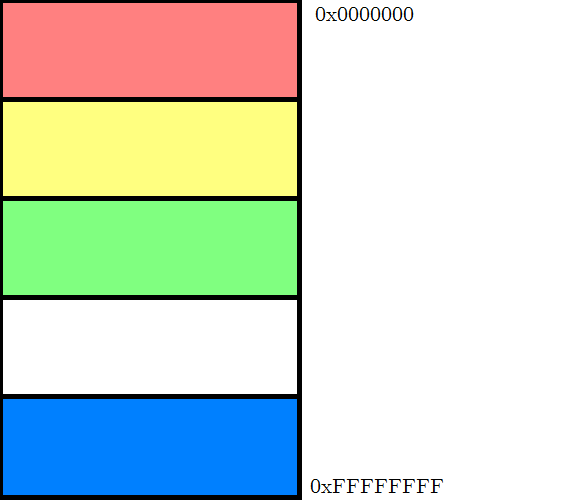
\includegraphics[width=50mm]{questions/programstructure.png}

\begin{answer}
red: text

yellow: data

green: heap

blue: stack
\end{answer}

		\section*{Modular Design}
		\item For each of the following snippets of code, state whether it should be placed in the header file (\texttt{.h}) or the source file (\texttt{.c}).

\begin{enumerate}

\begin{tabular}{p{.25in}p{1.5in} p{4.5in}}
\item
&
{
\begin{lstlisting}[numbers=none]
struct Point
{
	double x;
	double y;
};
\end{lstlisting}
}
&
\begin{answer}
Either. If the fields of the type need to be accessed from other source files, it must be defined in the header; otherwise, it only needs to be defined in the source file and possibly forward-declared or \texttt{typedef}'d in the header.
\end{answer}
\\
\item
&
{
\begin{lstlisting}[numbers=none]
int main(int argc, char **argv)
{
	int x = run_some_function();
	printf("%d\n", x);
	return 0;
}
\end{lstlisting}
}
&
\begin{answer}
\hspace{2.5in}
Source
\end{answer}
\\
\item
&
{
\begin{lstlisting}[numbers=none]
int do_something_and_return(int x, int y)
{
	if (y != 0)
		return x*y + (x/y);
	else
		return x*y;
}
\end{lstlisting}
}
&
\begin{answer}
\hspace{2.5in}
Source
\end{answer}
\\
\item
&
{
\begin{lstlisting}[numbers=none]
int do_something_and_return(int x, int y);
void do_something(int x, int y);
\end{lstlisting}
}
&
\begin{answer}
\hspace{2.5in}
Header
\end{answer}
\\
\end{tabular}
\end{enumerate}


		\section*{Abstract Data Types}
		\item 
Generally speaking, ADTs are easier to define and work with in procedural languages like C, as opposed to object-oriented languages like Java or C\#. (\textbf{True} or \textbf{False}). Explain your answer.

\begin{answer} 
\textbf{False}. C lacks object-oriented features that streamline the creation and use of ADTs in the language. C doesn't have access modifiers (e.g., \texttt{private} or \texttt{protected}), so hiding the underlying implementations is tougher, and will often involve the use of pointers.
\end{answer}

\item What is a \emph{primitive data type}? Provide 3 examples of primitive data types in C.

\begin{answer}
Primitive data types are supported by the language itself, as opposed to ones that are built from a combination of other objects (\emph{structured}), and ones that are extensions to the language (\emph{user-defined}). Examples include: \texttt{int}, \texttt{float}, \texttt{char}, \texttt{double}, \texttt{void}.
\end{answer}

\item Write a program that defines the structure of a queue:
\begin{itemize} {\small
	\item The queue ADT is described by its size (an unsigned int) and a pointer to the head/front of the queue.
	\item The queue is made up of nodes, which are each described by their value (any data type), and a pointer to the next node in the queue, or null if it is the last node in the queue.
	\item The queue's size describes the number of nodes present within the queue.
	\item The queue will support the following operations:}
	\begin{itemize} {\scriptsize
		\item A function which returns an int (0 or 1) representing whether or not the queue is empty, \texttt{int isEmpty(QueueADT q)}.
		\item A function which adds a new node onto the end of the queue, \texttt{void enqueue(QueueADT q, Node n)}.
		\item A function which removes the first node in the queue and returns it, \texttt{Node dequeue(QueueADT q)}.
		\item A function which returns an unsigned int representing the size of the queue, \texttt{unsigned int size(QueueADT q)}.}
	\end{itemize}
\end{itemize}

\begin{answer}
yolloooooo
\end{answer}




		\section*{Advanced C Features}
		\item \begin{enumerate}

\item Define a union, \texttt{typedef}ed to the name \texttt{printableData}, that can hold any of: an seven-character long string, a \texttt{double}, or an \texttt{int}.

\begin{answer}
\begin{verbatim}
typedef union {
    char stringData[8]; // 8 = 7 + NUL character
    double doubleData;
    int intData;
} printableData;
\end{verbatim}
\end{answer}

\item An idiom found in some C programs is the \textit{tagged union}. (Tagged unions are also commonly used in functional programming.)

\begin{verbatim}
typedef unsigned char tag_t;

// could also use an enum
const tag_t STRING_TAG = 0;
const tag_t DOUBLE_TAG = 1;
const tag_t INT_TAG = 2;

typedef struct {
    printableData data;
    tag_t tag;
} taggedData;
\end{verbatim}

In addition to the actual data, the tagged union stores a tag whose value corresponds to the type of data being stored. Because of this, we can tell which of the three types of values are being stored in the \texttt{data} field.\\
Write a function that takes an array of \texttt{taggedData} and prints out the data each element holds, each on its own line. Also take a \texttt{count} parameter. Assume all necessary headers have been included. (\textit{Hint:} Use a series of \texttt{if}/\texttt{else if} statements to properly print each type of data that can be stored.)

\begin{answer}
\begin{verbatim}
void printAll(taggedData* mixedArray, int count) {
    int i;
    for(i = 0; i < count; ++i) {
        if(mixedArray[i].tag == STRING_TAG) {
            printf("%s\n", mixedArray[i].data.stringData);
        } else if(mixedArray[i].tag == DOUBLE_TAG) {
            printf("%f\n", mixedArray[i].data.doubleData);
        } else if(mixedArray[i].tag == INT_TAG) {
            printf("%d\n", mixedArray[i].data.intData);
        }
    }
}
\end{verbatim}
\end{answer}
\newpage
\item Suppose that we want to be able to process this data in other ways besides just printing to standard out. We can use function pointers to write a more generic \texttt{processAll} function. Suppose the following struct is defined:

\begin{verbatim}
typedef struct {
    void (*processString)(char*);
    void (*processDouble)(double);
    void (*processInt)(int);
} processingFunctions;
\end{verbatim}

Define a \texttt{processAll} function that takes an array of \texttt{taggedData}, a \texttt{count} parameter, and a \texttt{processingFunctions} value, and uses the functions pointed to by the struct to process each element of the array, rather than using \texttt{printf} as was used in the \texttt{printAll} function.

\begin{answer}
\begin{verbatim}
void processAll(taggedData* mixedArray, int count, processingFunctions procs) {
    int i;
    for(i = 0; i < count; ++i) {
        if(mixedArray[i].tag == STRING_TAG) {
            (*procs.processString)(mixedArray[i].data.stringData);
        } else if(mixedArray[i].tag == DOUBLE_TAG) {
            (*procs.processDouble)(mixedArray[i].data.doubleData);
        } else if(mixedArray[i].tag == INT_TAG) {
            (*procs.processInt)(mixedArray[i].data.intData);
        }
    }
}
\end{verbatim}
\end{answer}
\end{enumerate}

% http://ideone.com/l4z5kP

		\item Suppose we have the following bit field representing a player in an role-playing game.

\begin{verbatim}
struct player {
    unsigned int alive:1;
    unsigned int gender:1;
    unsigned int class:2;
    unsigned int level:4;
};
\end{verbatim}

However, you need to store these players as 8 bit \texttt{unsigned char} values.
You decide to store \texttt{level} in the lowest 4 bits of the \texttt{unsigned char},
\texttt{class} in the next 2 bits,
\texttt{gender} in the next bit,
and \texttt{alive} in the highest bit.
Write a function that takes a \texttt{player} struct and
returns its \texttt{unsigned char} representation under the aforementioned rules.

\begin{verbatim}
unsigned char serializePlayer(struct player player1) {
\end{verbatim}
\begin{answer}
\begin{verbatim}
    // can also do a single return and `or` the values in one expression
    unsigned char data = 0;
    data |= player1.level;
    data |= player1.class << 4;
    data |= player1.gender << 6; // 4 + 2
    data |= player1.alive << 7; // 4 + 2 + 1
    return data;
\end{verbatim}
\end{answer}
\begin{verbatim}
}
\end{verbatim}


		\section*{OS-Level I/O}
		\item Explain the relationship between the FD table, the open file table, and the I-node table. Which tables are in user space (a.k.a. private kernel space) and which are in system space (a.k.a. shared kernel space).

\begin{answer}
Each process has its own FD table, which are indexed by the file descriptors returned by functions like \texttt{open}.
Among other things, they hold a file pointer which refers to an entry in the open file table.
The open file table is shared by all processes and holds data about all currently open files.
A new entry is created in the open file table each time \texttt{open} is called by a C program,
even if that same file is currently open in another process.
The data it holds includes the current offset, as well as a pointer to an entry in the I-node table.
The I-node table is also shared by all processes,
but it has exactly one entry for each file in the file system,
whether that file is open or not;
the data stored in the table includes things like file permissions.
The FD table is in user space, while the open file table and the I-node table are in system space.
\end{answer}

		\item You create a file named \texttt{sliding.txt} with the following contents (there are newlines between each line, but not at the end of the file):

\begin{verbatim}
>>>>v
>>>>v
>>>>v
>>>>v
>>>>v
\end{verbatim}

However, your no-good friend sneakily changes one of the lines to \begin{verbatim}^<<<<\end{verbatim} and you don't know which line it is. Write a program that fixes the file, but only writes 5 characters (it can read the whole file, however). Do not worry about error handling. (\textit{Hint:} You can use the \texttt{strstr} function in \texttt{<string.h>}, which takes two strings, searches for the second string inside the first, and returns the \texttt{char*} location within the first string where the second string was found. You may also need pointer arithmetic.)

\begin{answer}
\lstinputlisting{code/os_io_sliding_tiles.c}
\end{answer}

		\newpage
		\section*{Threads \& Processes}
		\item Describe the differences between programs, processes, and threads.

\begin{answer}
Program - instructions on disk, static

Process - the executing program

Thread - instruction execution stream of a process
\end{answer}


	\end{enumerate}
\end{document}
